\documentclass[tikz]{standalone}
\usepackage{tikz}
\usepackage{pgfplots}
\usetikzlibrary{shapes,arrows,positioning}
\begin{document}
% Define block styles
\tikzstyle{decision} = [diamond, draw, fill=yellow!10, 
    text width=4.5em, text badly centered, node distance=2cm, inner sep=0pt]
\tikzstyle{block} = [rectangle, draw, fill=blue!20, 
    text width=2.8cm, text centered, minimum height=4em]
\tikzstyle{line} = [draw, -latex']
\tikzstyle{inout} = [draw, trapezium,
    trapezium left angle = 65,
    trapezium right angle = 115,
    trapezium stretches,fill=green!20, node distance=4cm,
    minimum height=2em, text width=1.7cm]
\tikzstyle{startend} = [rounded rectangle, draw, fill=red!20, 
    text width=2.6cm, text centered, minimum height=4em]
    
    
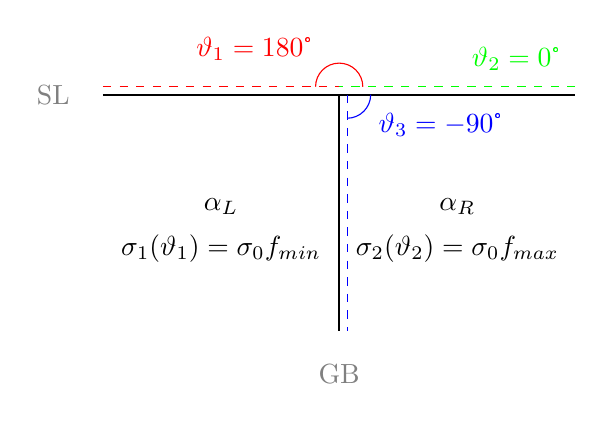
\begin{tikzpicture}
    \def\dim{3}
    \draw[thick] (-\dim,0) -- (\dim,0);
    \draw[thick] (0,-\dim) -- (0,0);
    % \draw node at (1.5*\dim,1.5*\dim) {$n_C$};
    
    \draw node[below] at (0.5*\dim,-0.4*\dim) {$\alpha_R$};
    \draw node[below] at (0.5*\dim,-0.55*\dim) {$\sigma_2(\vartheta_2)=\sigma_0f_{max}$};
    
    \draw node[below] at (-0.5*\dim,-0.4*\dim) {$\alpha_L$};
    \draw node[below] at (-0.5*\dim,-0.55*\dim) {$\sigma_1(\vartheta_1)=\sigma_0f_{min}$};
    
    \draw[red,dashed] (-\dim,0.1) -- (0,0.1);
    \draw[green,dashed] (\dim,0.1) -- (0,0.1);
    % \draw[red] node at (-0.75*\dim,0.15*\dim) {};
    \draw[red] (0.3,0.1) arc (0:180:0.3cm) node[near end,above left] {$\vartheta_1=180$\textdegree};
    \draw[green] node at (0.75*\dim,0.15*\dim) {$\vartheta_2=0$\textdegree};
    
    \draw[blue,dashed] (0.1,0) -- (0.1,-\dim);
    \draw[blue] (0.3+0.1,0) arc (0:-90:0.3cm) node[near start,below right] {$\vartheta_3=-90$\textdegree};
    
    \draw[gray] (0,-1.1*\dim) node[below] {GB};
    \draw[gray] (-1.1*\dim,0) node[left] {SL};
    
\end{tikzpicture}

\end{document}